\section{Backend - REST-Schnittstelle und Infrastruktur}
	\subsection{Überblick}
	Das Backend besteht aus mehreren Komponenten. Einerseits muss eine gewisse Software-Infrastruktur aufgebaut werden, um \Gls{webinterface} und die REST-Schnittstelle bereitzustellen. Andererseits muss die Anwendung selbst auch entwickelt werden. Diese besteht wiederum auch aus mehreren Teilen. Darunter fällt die REST-Schnittstelle, inklusive der implementierten Endpoints, selbst, Schnittstellen zu diversen Diensten, wie dem TGM-LDAP Server, zur Datenbank, zu Google Maps und zu WebUntis, aber auch die weitere Funktionalität der Anwendung, unter anderem das Versenden von E-Mails oder Erstellen von PDF-Dateien.
	\\
	\begin{figure}[H]
		\centering
		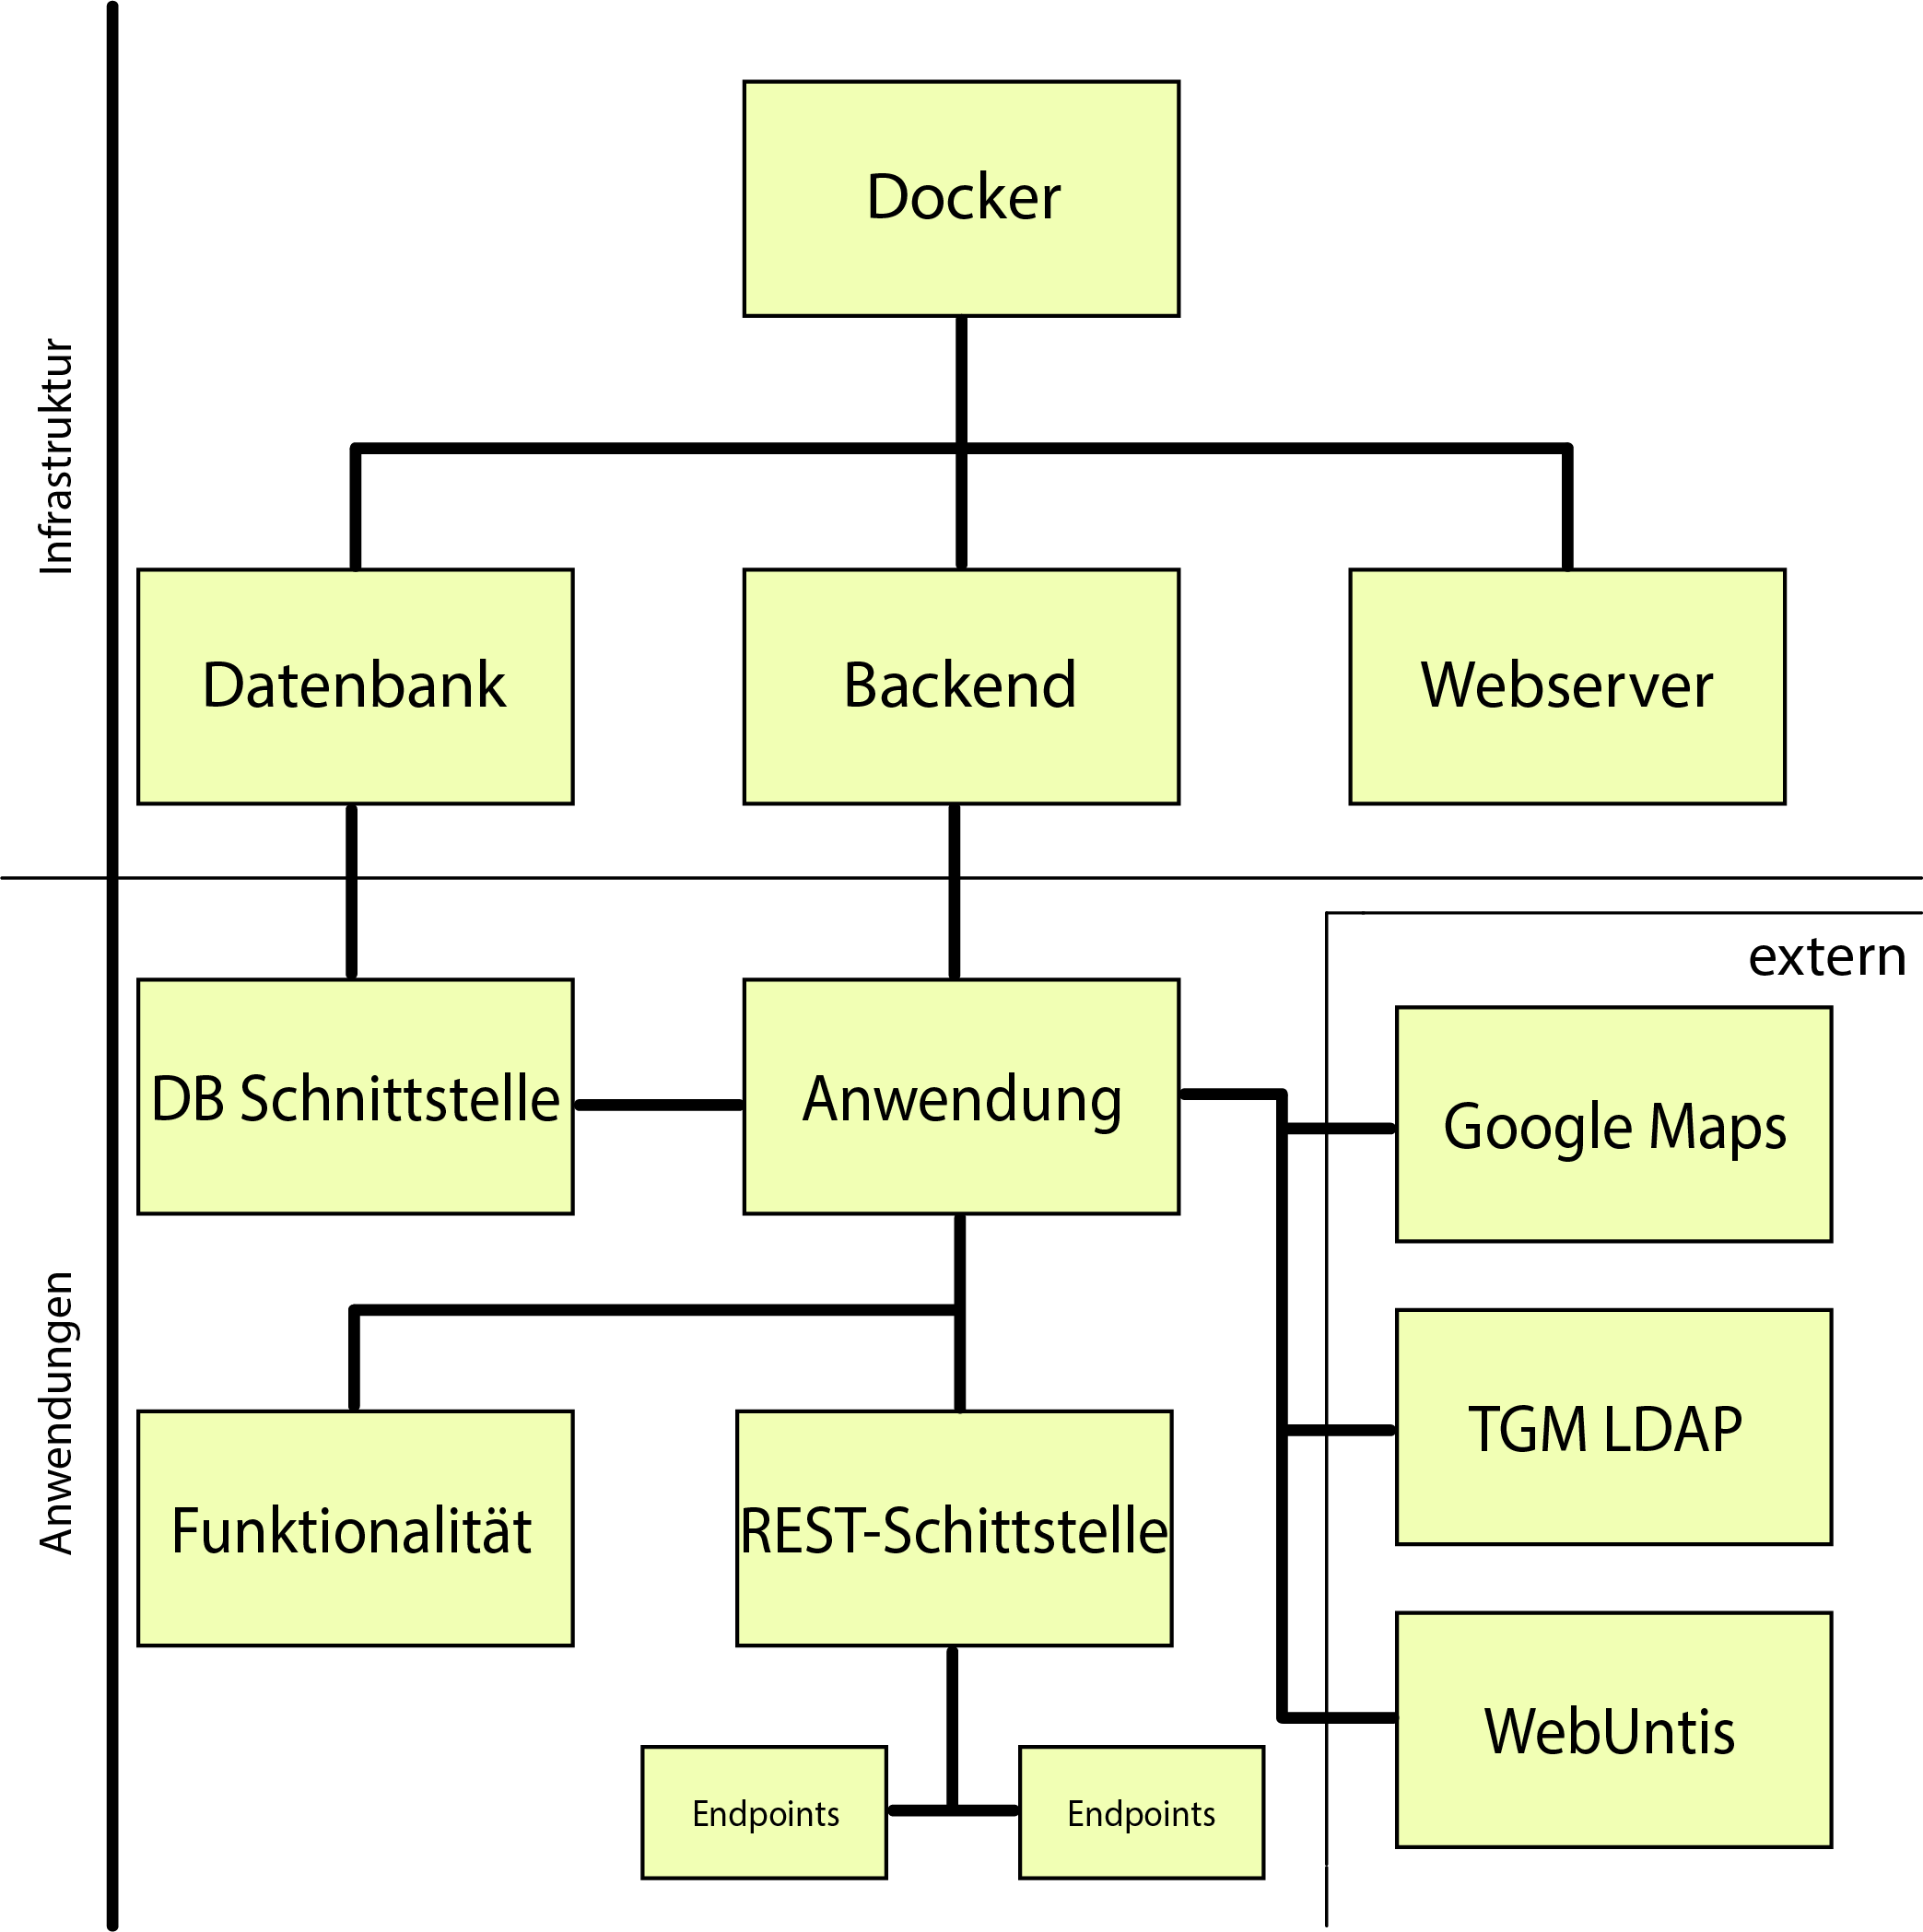
\includegraphics[width=0.8\linewidth]{images/uebersicht}
		\caption[Übersicht über die Komponenten]{Übersicht über die verschiedenen Komponenten der Infrastruktur und der Anwendung}
		\label{fig:uebersicht}
	\end{figure}
	
	\subsection{Docker}
	Um die Infrastruktur des Projektes einfach aufbauen zu können, wird \Gls{docker} genutzt. Da es sich hier um eine komplex strukturierte Infrastruktur handelt wird zusätzlich das Werkzeug \Gls{dcompose} genutzt.
		\subsubsection{Datenbank}
		\subsubsection{Backend-Container}
		\subsubsection{Webserver}
	\subsection{Deployment}
	\subsection{REST-Schnittstelle}
		\subsubsection{Framework}
		\subsubsection{Endpoints}
	\subsection{Funktionalität}
		\subsubsection{TGM-LDAP Schnittstelle}
		\subsubsection{Datenbank Schnittstelle}
		\subsubsection{Google Maps}
		\subsubsection{WebUntis}
		\subsubsection{E-Mails}
		\subsubsection{PDF-Dateien}
	\subsection{Kommunikation und Datenformate}